\begin{figure}[htp]
  \centering
  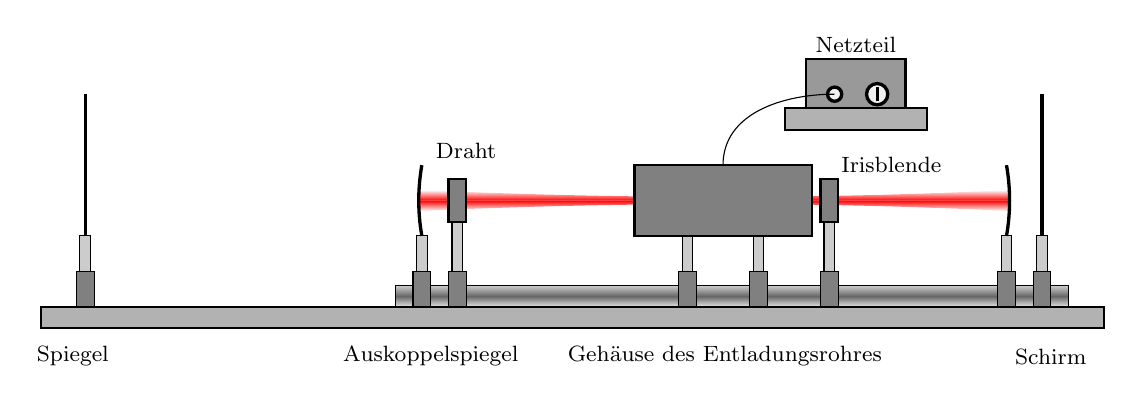
\begin{tikzpicture}[scale=0.9]

    \shadedraw[top color =black!20!white, bottom color=black!10!white, middle color=black!60!white] (-1.5,0) rectangle (8,0.3);
    \filldraw[thick, draw = black, fill=black!30!white] (-6.5,0) rectangle (8.5,-.3);

    \shade[top color=white, bottom color=red] (3.125,1.5) parabola bend (3.125,1.55) (-1.17,1.65) -- (-1.17,1.5);
    \shade[top color=red, bottom color=white] (3.125,1.5) parabola bend (3.125,1.45) (-1.17,1.35) -- (-1.17,1.5);
    \shade[top color=white, bottom color=red] (3.125,1.5) parabola bend (3.125,1.55) (7.18,1.65) -- (7.18,1.5);
    \shade[top color=red, bottom color=white] (3.125,1.5) parabola bend (3.125,1.45) (7.18,1.35) -- (7.18,1.5);
    \filldraw[draw=black, fill=gray] (-6,0) rectangle +(0.25,0.5);
    \filldraw[draw=black, fill=black!20!white] (-6+0.05,0.5) rectangle +(0.15,0.5);
    \draw[very thick] (-6+0.125,1) -- +(0,2);
    \filldraw[draw=black, fill=gray] (7.5,0) rectangle +(0.25,0.5);
    \filldraw[draw=black, fill=black!20!white] (7.5+0.05,0.5) rectangle +(0.15,0.5);
    \draw[very thick] (7.5+0.125,1) -- +(0,2);

    \filldraw[draw=black, fill=gray] (-1.25,0) rectangle +(0.25,0.5);
    \filldraw[draw=black, fill=black!20!white] (-1.25+0.05,0.5) rectangle +(0.15,0.5);
    \draw[very thick] (-1.25+0.125,1) arc (190:170:3-0.125);

    \filldraw[draw=black, fill=gray] (2.5,0) rectangle +(0.25,0.5);
    \filldraw[draw=black, fill=black!20!white] (2.5+0.05,0.5) rectangle +(0.15,0.5);
    \filldraw[draw=black, fill=gray] (3.5,0) rectangle +(0.25,0.5);
    \filldraw[draw=black, fill=black!20!white] (3.5+0.05,0.5) rectangle +(0.15,0.5);
    \filldraw[thick, fill=gray, draw=black] (1.875,1) rectangle +(2.5,1);

    \filldraw[draw=black, fill=gray] (4.5,0) rectangle +(0.25,0.5);
    \filldraw[draw=black, fill=black!20!white] (4.5+0.05,0.5) rectangle +(0.15,0.9);
    \filldraw[thick, fill=gray, draw=black] (4.5,1.2) rectangle +(0.25,.6);

    \filldraw[draw=black, fill=gray] (-0.75,0) rectangle +(0.25,0.5);
    \filldraw[draw=black, fill=black!20!white] (-0.75+0.05,0.5) rectangle +(0.15,0.9);
    \filldraw[thick, fill=gray, draw=black] (-0.75,1.2) rectangle +(0.25,.6);

    \filldraw[draw=black, fill=gray] (7,0) rectangle +(0.25,0.5);
    \filldraw[draw=black, fill=black!20!white] (7+0.05,0.5) rectangle +(0.15,0.5);
    \draw[very thick] (7+0.125,1) arc (-10:10:3-0.125);

    \filldraw[thick, draw = black, fill=black!30!white] (4,2.5) rectangle (6,2.8);
    \filldraw[thick, draw = black, fill=black!40!white] (4.3,2.8) rectangle (5.7,3.5);
    \draw[fill=black!5!white, very thick] (4.7,3) circle (.1cm);
    \draw[fill=black!5!white, very thick] (5.3,3) circle (.15cm);
    \draw[very thick] (5.3,3.1) -- (5.3,2.9);
    \draw (4.7,3) to[out=180,in=90] (3.125,2);

    \node (A) at (5.5,2){\footnotesize Irisblende};
    \node (A) at (3.15,-.7){\footnotesize Gehäuse des Entladungsrohres};
    \node (A) at (7.75,-.7){\footnotesize Schirm};
    \node (A) at (-1,-.7){\footnotesize Auskoppelspiegel};
    \node (A) at (-6.05,-.7){\footnotesize Spiegel};
    \node (A) at (-.5,2.2){\footnotesize Draht};
    \node (A) at (5,3.7){\footnotesize Netzteil};
  \end{tikzpicture}
  \caption{Schematischer Aufbau des Gaslasers.}
  \label{fig:Laseraufbau}
\end{figure}
